\chapter{Literature Review}
\label{ch:lit}

%TODO: Diagram - What issues do I cover, how are they linked? Soundscape practice, Acoustic Analysis, Predictive Modelling
%TODO: Content from Soundscape and the Built Environment, Chapter 10, Applied Soundscape Practice

% \section{Impact of Urban Noise on Health and Wellbeing}

% \cit{Environmental noise in Europe 2020}

% \draft{Give a brief background to why noise control is important for public health.}
% % https://www.euro.who.int/__data/assets/pdf_file/0008/383921/noise-guidelines-eng.pdf?ua=1

% \section{Current Methods of Assessing and Addressing Urban Noise}

% The approach to a practical predictive soundscape model arrived at within this thesis is heavily based on past environmental acoustics approaches. I will therefore begin with a brief summary of these past approaches.

% \subsection{Acoustical Parameters}

% \subsection{ISO Environmental Acoustics Standards}
% \cit{ISO 1996-1, esp sections on annoyance, e.g. Annex F, G, H}

% \subsection{EU Noise Mapping}

% \cit{Environmental noise in Europe 2020}

% \subsection{Shortcomings}


\section{Soundscape Studies}

\subsection{Soundscape Descriptors and Indices}


\subsection{Standardisation}
% From: Protocol paper
The soundscape community is undergoing a period of increased methodological standardization in order to better coordinate and communicate the findings of the field. This process has resulted in many operational tools designed to assess and understand how sound environments are perceived and apply this to shape modern noise control engineering approaches. Important topics which have been identified throughout this process are soundscape 'descriptors', 'indicators', and 'indices'. \citet{Aletta2016Soundscape} defined soundscape descriptors as "measures of how people perceive the acoustic environment"; soundscape indicators as "measures used to predict the value of a soundscape descriptor; soundscape indices can then be defined as "single value scales derived from either descriptors or indicators that allow for comparison across soundscapes" \citep{Kang2019Towards}.

This conception has recently been formalized and expanded upon with the adoption of the recent ISO 12813 set of standards \citep{ISO12913Part1, ISO12913Part2,ISO12913Part3}. ISO 12913 Part 1 sets out the definition and conception of Soundscape, defining it as the "acoustic environment as perceived or experienced and/or understood by a person or people, in context". Here, the soundscape is separated from the idea of an acoustic environment, which encompasses all of the sound which is experienced by the receiver, including any acoustically modifying effects of the environment. In contrast, the soundscape considers the acoustic environment, but also considers the impact of non-acoustic elements, such as the listener's context and the visual setting, and how these interact with the acoustic environment to influence the listener's perception.

\subsection{Soundscape Descriptors}
In order to consistently discuss soundscape and the factors which influence it, it is important to understand what terms have been used to describe soundscapes and to construct a consistent framework within which to work. Both the traditional focus on the epidemiological impacts of noise and the development of the soundscape concept have used many different terms in order to describe the perception of a sound environment.

\paragraph{Noise annoyance} is perhaps the best researched aspect of environmental sound perception.

\paragraph{Pleasantness}

\paragraph{Quietness / Tranquillity}

\paragraph{Acoustic Comfort}

\paragraph{Perceived sound level}

\paragraph{Music-likeness}

\paragraph{Restorativeness}

\paragraph{Soundscape quality}

\paragraph{Appropriateness}

\paragraph{Perceived Affective Quality (PAQ)}

\subsection{Soundscape Indicators}
% From: Protocol paper
Several studies prior to the formalization of the ISO standards on soundscape demonstrated the general, but inadequate, relationship between traditional acoustic metrics, such as $L_{Aeq}$, with~the subjective evaluation of the soundscape \citep{Berglund2006Tool,Yang2005Acoustic,Rychtarikova2013Soundscape,Aumond2017Modeling,AlsinaPages2021Perceptual}. These have typically aimed to address the existing gap between traditional environmental acoustics metrics and the experience of the sound environment. Yang and Kang (2005) showed that, when the sound level is 'lower than a certain value, say 70 dBA', there is no longer a significant change in the evaluation of acoustic comfort as the sound level changes. However, the perceived sound level does continue to change along with the measured sound level, showing that (1) measured sound level is not enough to predict soundscape descriptors such as 'acoustic comfort', and (2) there is a complex relationship between perceived sound level and soundscape descriptors which is mediated by other factors.

Subsequent studies have shown that, even with large data sets and several possible acoustic indicators examined, models that are based on objective/measurable metrics under-perform in predicting soundscape assessment when compared to models based on perceptual responses. \citet{Ricciardi2015Sound}, with a methodology based on smart phone recordings, achieved $R^2 = 0.21$ with acoustic input factors $L_{50}$ and $L_{10} - L_{90}$, whereas the same dataset and model building method achieved $R^2 = 0.52$ with perceptual input factors overall loudness (OL), visual amenity (VA), traffic (T), voice (V), and birds (B). This indicates that merely examining the acoustic level is not sufficient for predicting the assessed soundscape quality, and that additional objective factors and a more holistic and involved method of characterizing the environment is required. These previous studies have generally been limited by one or many of the following factors:

\begin{itemize}
  \item limited number or types of locations;
  \item limited responses sample size;
  \item no non-acoustic factors.
\end{itemize}
These factors generally limit the generalizability of their results beyond the investigated locations.

\subsection{The need for predictive soundscape models}
%TODO: Probably need to combine and rephrase with "Practical Applications for Soundscape Mapping""
% From: Protocol paper
The ability to predict the likely soundscape assessment of a space is crucial to implementing the soundscape concept in practical design. Current methods of assessing soundscapes are generally limited to a post-hoc assessment of an existing environment, where users of the space in question are surveyed regarding their experience of the acoustic environment \citep{Engel2018Review, Zhang2018Effect}. While this approach has proved useful in identifying the impacts of an existing environment, designers require the ability to predict how a change or proposed design will impact the soundscape of the space. To this end, a model that is built upon measurable or estimate-able quantities of the environment would represent a leap forward in the ability to design soundscapes.

Developing soundscape indices is a process that requires consideration of how people perceive, experience, and understand the surrounding sound environment. For the purpose of modelling and comparisons,

% ? Replace with section from Protocol paper?
Previous soundscape research has demonstrated that perception of the acoustic environment, while primarily driven by sound level, is mediated heavily by non-acoustic factors which interact with the sound level, spectral information, and temporal acoustic behaviour in complex ways. The soundscape is influenced by several levels of factors: the immediate and long-term acoustic environment, other environmental factors (e.g. temperature, air quality), the physical / visual characteristics of the space, the type of architectural space, and even cultural and country-level expectations. When approached in a predictive model context, the acoustic data must form the core components, but a coherent framework for describing how the influence of the acoustic factors is affected by the non-acoustic factors is required.

Simpler analyses have taken a fragmented approach, for instance where separate acoustic-factor models are built independently for each type of architectural space considered in the data set and, separately, statistical models are built to investigate another non-acoustic factor, e.g. visual greenness vs lack of greenness. In order to properly extract the influences of all of these levels of factors as well as to build a generalisable model which can be used in practice, this fragmented approach should be combined into a single multi-level model.

% From: Turing application proposal
The first key step for this approach is the creation of a coherent, large-scale, multi-factor database of objective environmental measurements and subjective perceptual responses. My research makes use of in-person field questionnaires, long-term manned questionnaires, and multi-factor characterisation of the environment as part of the ERC-funded project Soundscape Indices (SSID) and in collaboration with The French Institute of Science and Technology for Transport, Development and Networks (IFSTTAR) to collect this database across a wide range of locations and soundscape types. This work has already been mostly completed and the database is now ready to be put to use in building the overall soundscape predictive model.

This approach is unique in that it:
\begin{enumerate}
  \item fundamentally incorporates all identified factors of soundscape perception in a coherent manner;
  \item is extensible and interpretable;
  \item considers how soundscape change over both multi-hour and multi-day timescales and incorporates this dynamic behaviour for increased accuracy.
\end{enumerate}

%NOTE: In contrast to Lacey
Where previous ground-breaking strategies toward practical urban soundscape design \citep{Lacey2019Noise}, have been limited in their scope, providing methods of improving individual soundscapes or approaches which can be applied to bespoke projects, this work aims to move towards a generalised and widely applicable engineering-based approach. The goal is to promote a soundscape mindset as the 'standard', not just as an extra add-on for forward-thinking projects or as a localised sonic rupture which, while incredibly effective (and affective) within its radius, is not suited to being applied on a city- or national-policy scale. For this purpose, we require a standardised and implementable index and direction of best practice which can be implemented by trained technicians, engineers, designers, and planners across all aspects of urban design, from the billion dollar museum to the inner-city public elementary school. A desire for good and restorative soundscapes should be the baseline standard in a city's design, upon which art which highlights the 'mythic, imaginative and poetic relationships within the affective environments' \citep{Lacey2019Noise} can be implemented by the specialists. The goal of this work therefore, is not to critique or counter the creative approaches taken by those within sound art or acoustic ecology, but instead to move towards a new baseline, a new way of designing all environments of the city, from the lowest to the highest (but mostly at the lowest, where it is needed most).



\subsection{Demographic differences}
Several studies have attempted to study the degree to which personal and demographic factors influence a person's soundscape perception. In some conceptions \cit{Kou2020effects} % CITE add Erfanian 2020
these personal factors are classed as 'contextual' soundscape indicators - features which influence or, in a modelling context, be used as independent variables to predict the value of a soundscape descriptor. The personal factors help to create a personal soundscape interpretation model which is individual to each person.

In this way, a person's individual state-of-mind, ethnic identity, educational background, gender identity, etc. form a pseudo-deterministic framework %! what a load of crap
through which the physical inputs from their environment are filtered. Clearly, many of these personal factors could never be measured and even those which are measurable will have wide ranges of legitimate effects, however estimating the degree and type of effect they may have can both help us better predict individual soundscape assessments and understand how group identities influence sound perception.

%TODO: Need to include earlier, more foundational studies into demographic factors

\paragraph*{Section on Erfanian et al. 2020, Psychological Well-being}

\paragraph*{Low-income and minority evidence} % FIXME I think this section will need to be heavily revised for phrasing and content. I'm not happy with how I'm discussing under-represented groups.
A consistent limitation of soundscape studies investigating the influence of personal factors is a sampling bias towards majority ethnicities (typically White British for UK studies and ethnic Chinese for Chinese studies) and middle-class and highly educated groups. % CITE Hoo boy citation definitely needed
This results in not only incomplete information about how demographics influence soundscape perception, but also represents a systemic under-representation of certain environments. While it may be unclear to what extent ethnicity and social class internally influence a person's perception, it is clear that these groups are exposed to different sound environments % NOTE: socio-economic studies - Huan 2019? Jian ~2015?, Environmental noise in Europe 2020

and therefore studies which do not include under-represented groups are also by definition not including those sound environments which those groups inhabit.

A recent study by \cit{Kou2020effects} was successful in making inroads in these under-represented environments by studying the Humboldt Park neighbourhood in Chicago, USA. Their study included
% TODO: Finish summarising results from Kou2020


\section{Approaches to Soundscape in Engineering}

From this literature review, some conclusions about current approaches to incorporating the concept of "soundscape" into practical engineering and architectural design have been identified.

\subsection{The Quiet Areas approach}

This approach maintains a focus on "identifying and preserving quiet areas" \citep{EEA2020Environment} following the imperative given in the \gls{end} \citep{EU2002Directive}. This approach is mostly rooted in a noise mindset, although the methods employed for identifying quiet areas vary across countries within the EEA. Background sound levels seem to play an important role in identifying quiet areas, in particular when attempting to produce maps of available quiet areas on a city- or agglomeration-scale such as that used in the \citet{EEA2020Environment}, where quiet areas were defined as: "those with less than 55 dB $L_{den}$ from road, rail, aircraft and industrial sources and were classified, depending on their land cover type, as quiet areas with green/blue land cover." However, several background noise thresholds are cited as being used by agglomerations for their definitions, along with non-acoustic criteria such as urban functionality, land cover type, location, size and accessibility of the area, visual qualities, and subjective judgement. %CITE: pg 70 EnE
Despite these attempts to incorporate multiple factors within the definition of quiet areas, this approach still tends toward a 1- or 2-dimensional focus, and struggles to take a holistic approach to people's perception or response to the space.

Given that the Quiet Areas approach started with the 2002 \gls{end}, predating the ISO 12913 series of technical specifications on soundscape, it has not yet moved in line with the conception of "soundscape" and the accompanying measurement methods and reporting requirements given in the ISO documents. There is therefore an open question of whether the directive to identify and preserve quiet areas would truly be considered soundscape, however it does represent the most successful foray into policy and is frequently cited as a success by soundscape researchers \cit{Aletta, Guastavino, Kang, etc.}.

\subsection{SSID approach}

\subsection{Qualitative / Community approach}
\draft{An approach rooted in the qualitative and sociological relationships between people and their soundscapes. Focus on Sarah Payne and Edda Bild's work. }

\subsection{Sound Art / Installations}

These merit a necessary mention, however sound art and installations are typically considered distinct from 'engineering' and are not employed at every project. Therefore, these are not discussed further as their own approach, distinct from the other, more engineering-applied approaches. 

%TODO: Need to read/write a lot more on this. Focus on 

%TODO Continue adding from Remarkable notes

\section{Existing Predictive Models}

Contrary to the hopes expressed by \citet{Aletta2014Towards}, that "ideally there should be one acoustic indicator per dimension", the evidence from subsequent investigations and modelling attempts \citep{Lionello2020systematic} indicates this to be unlikely. There appears to be no reason we should think the perceptual dimensions should be reduced to a single acoustic indicator. The dimensions of soundscape represent complex perceptual concepts which we should expect to be composed of a multi-factor interaction between the input features. This necessary complexity  highlights the need for a more sophisticated machine learning approach in order to handle and interpret the interactions between the many input features which contribute to the formation of a soundscape perception.
\citep{Aletta2016Soundscape}

\citep{Lionello2020systematic}

\subsection{Models based on non-acoustic data sources}

\citep{Verma2020Predicting}, \citep{Gasco2020Social}

\subsection{Red and Green Soundscape Indices}
\citep{Yang2022Effects,Kogan2018Green} 

\subsection{Clustering/Classification Approach}
%FIXME: Probably needs to go to a new location
%TODO: Review Sun 2019 Classification
One approach which may seem promising is to generate clusters of soundscapes. \draft{Review ref on this -> \citet{Sun2019Classification}}. Soundscape perception of a space has many dimensions and can be difficult to adequately express. Clustering analysis provides a method to investigate the patterns present in a high-dimensional dataset and aid interpretation while imposing minimal starting assumptions. Within soundscape, this would enable the identification of 'soundscape types' based on some combination of perceptual, physical, and architectural data. 

For the purposes of predictive soundscape modelling with the characteristics laid out above, clustering would allow us to identify perceptual types, into which a soundscape could be placed based on its physical features. This process is outlined in \cref{fig:clusterModel}. Once the combined perceptual, contextual, and physical data are collected, unsupervised clustering analysis is performed on the perceptual data, including all \gls{paq}s, the overall questions, and perhaps demographic data. Once the clusters are identified. prior knowledge and information about the architectural typologies and use cases are used to inform the selection of appropriate descriptive labels for the clusters. Then... %TODO: Continue clustering discussion.

\begin{figure}
  %TODO: Create clustering approach model
  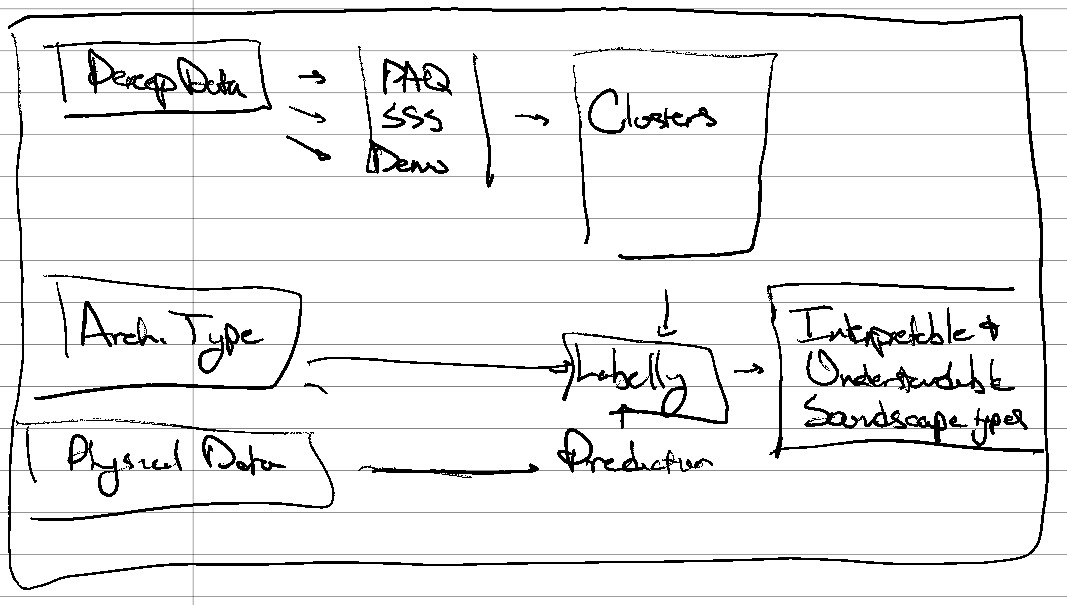
\includegraphics[width=\textwidth]{Figures/Remarkable clustering figure.jpg}
  \caption{Draft figure of a clustering approach}\label{fig:clusterModel}
\end{figure}

\draft{Issue with this approach to expand on: Limitations of starting dataset - impossible to know if we've identified all possible classes. Highly dependent on the primary dataset, the identified clusters cannot extend beyond what was already present.}